%TEX root = ../dissertation.tex

\chapter{Implementation}
\label{chapter:implementation}
In chapter \ref{chapter:solution}, we have presented the solution, that is,
the mobile apps that owners and end users need and the API that developers use
to develop proximity-based mobile apps for this two kinds of users.
Here, it will be explained the implementation of each part of the solution
(tools, programming languages, etc). Since there are two examples that were
created to test the concept, we will dive into their implementation also.
The code is hosted on
github\footnote{http://github.com/}, which is a hosting service for projects
that use git\footnote{http://git-scm.com/}, as their \gls{VCS}.

The technology chosen to support the proximity-based behaviour was
\gls{BLE} Beacons.
We have used three beacons from Estimote\footnote{http://estimote.com}
(figure \ref{fig:estimote}), that come with a development kit.
Besides the hardware, this product offers a \gls{SDK} for Android and
iOS. It also has a cloud service where developers can set and get
some information about each beacon, such as, the \gls{UUID}, name, etc.
% Photo of the three beacons

\begin{figure}[!ht]
  \centering
    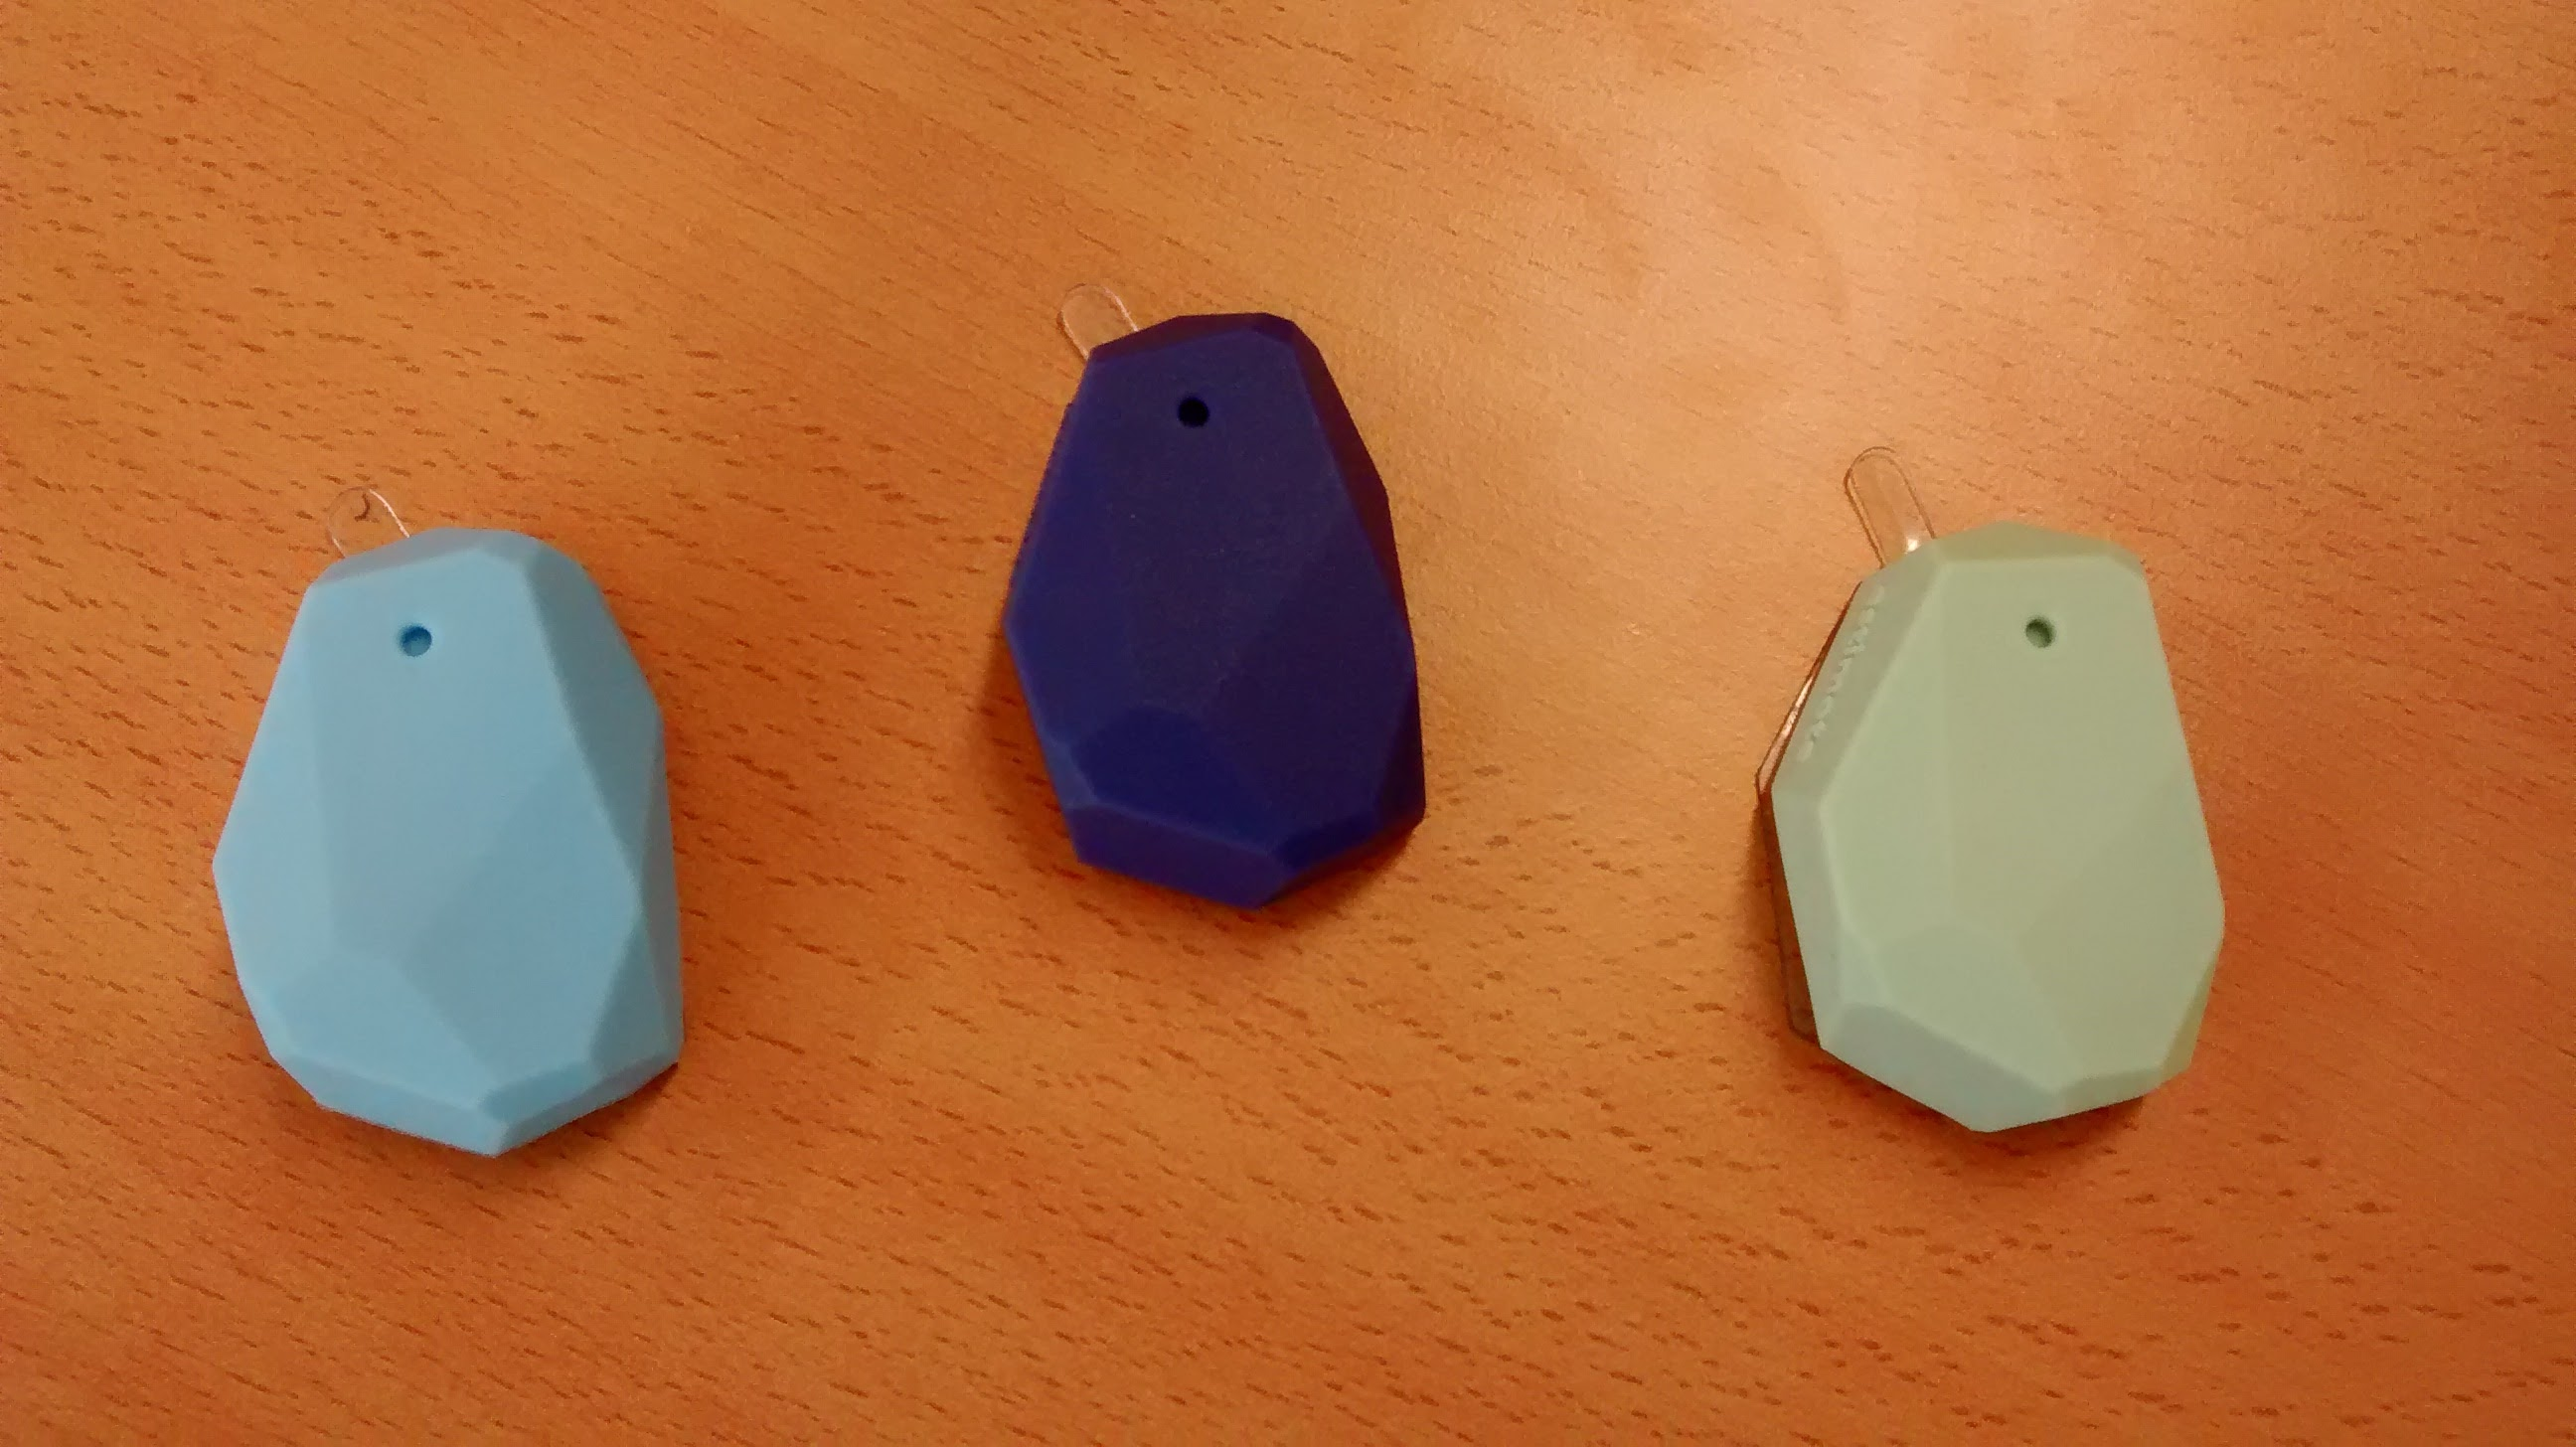
\includegraphics[width=0.5\textwidth, keepaspectratio]{images/estimote}
    \caption{Beacons from Estimote, that were used during the implementation}
    \label{fig:estimote}
\end{figure}

\section{Backend}
\label{sec:backend}
% BaaS, Parse.com
% What it is
% How it works
% Collections created (UML?)
% SDKs used
Since this solution needs to store information about each beacon, we
needed a backend to be able to change this information without having
to change the mobile apps.
However, this backend just had to be able to store data and retrieve that
data when client applications request it.
Instead of implementing this component from the scratch, we used
Parse\footnote{https://parse.com}, which is a \gls{BaaS}.
It gives, to developers, a dashboard, where they can create classes
and define their fields and the type of each field, which can be a string,
a number, a boolean, a pointer to another object, a \gls{JSON} object, etc.
In order to support the needs of this project, the following classes were
created, according to the data model in figure \ref{fig:backend_data_model}:
\begin{description}
  \item[Beacon]: Stores the information according to ibeacon protocol,
  which is \gls{UUID}, major and minor values. It also has a pointer
  to an instance of class User (already provided by Parse.com),
  which represents the user that owns the beacon;
  \item[Smart Place]: Stores information all smart places available,
  such as, name and description. It has a pointer to an instance of
  User, which is the user that created it;
  \item[Smart Place Instance]: When an owner wants to install a given
  Smart Place, he creates an instance of a Smart Place. Owners can
  customize the title and the message that appears in the users'
  mobile devices notifications;
  \item[Tag]: A Tag has a \gls{JSON} object and has pointers to instances
  of Smart Place Instance and Beacon classes. With this pointers, when
  the end users app detects a beacon, it is possible to send a query to
  the backend in order to get the tag that is associated to that beacon.
\end{description}

\begin{figure}[!ht]
  \centering
    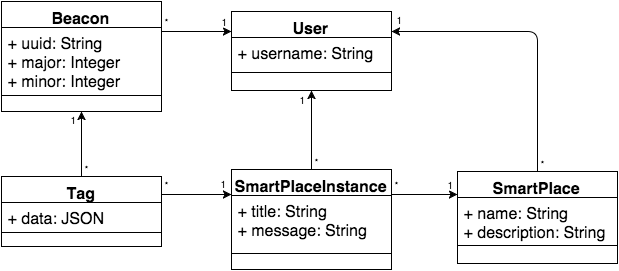
\includegraphics[width=0.5\textwidth]{images/backend_data_model}
    \caption{Data model stored in Parse \gls{BaaS}}
    \label{fig:backend_data_model}
\end{figure}

Parse \gls{BaaS} has \glspl{SDK} available to many platforms and programming
languages, such as, Android, iOS, Javascript, etc.
In order to be able to make requests to the backend from the mobile apps and
from the Javascript API
the Parse Android and Javascript \glspl{SDK} were used.

\section{Mobile applications}
\label{sec:mobile_applications}
% Mobile apps: Tools used, programming languages,
% -> Some kind of UML for each one
There is a mobile app for owners and another one for end users.
Each of these apps is an Android app. They were developed using Android
Studio, which is an \gls{IDE}, based on
IntelliJ\footnote{https://www.jetbrains.com/idea/},
to develop Android
applications and written in JAVA.
The chosen development environment allows developers to create multiple
apps and modules inside the same project.
Taking that into account,
one project was created, with 2 apps and one library, as shown in figure
\ref{fig:smartplaces_package}. Since both apps use the Bluetooth receiver
of the mobile device and make requests to the backend, there is a library,
that both apps depend on, that offers some abstractions around the ibeacon
protocol and the communication with Parse.
Its implementation is detailed in section \ref{sub:library}

\begin{figure}[!ht]
  \centering
    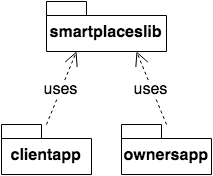
\includegraphics[width=0.5\textwidth, height=0.15\textheight,
      keepaspectratio]{images/smartplaces_package}
    \caption{Android project's structure}
    \label{fig:smartplaces_package}
\end{figure}

\subsection{Library}
\label{sub:library}
% Explain what the lib does
% UML for the lib
% Examples of its usage
As already mentioned, a library, smartplaceslib, as shown in figure \ref{fig:smartplaces_package}, was created in order to provide \glspl{API} that mobile apps can
use. Because, both apps use the Bluetooth receiver and interact with the backend, this library avoids having similar code in both apps. There are two important classes that this library offers:
\begin{description}
  \item[IBeaconsManager]: Offers methods to start scanning for beacons and change some settings such as, interval between each scan;
  \item[AbstractParseDataStore]: This class offers an abstraction of the Parse Android \gls{SDK}. It is extended by two classes, ClientParseDataStore, used in the end users mobile app, and OwnerParseDataStore, used in the owners mobile app. There are two different classes for each app because each app has different needs when interacting with the backend. There were common needs encapsulated in methods in the AbstractParseDataStore class.
\end{description}

When IBeaconsManager class is used, it needs a BeaconScanCallback object, which overrides a method that is executed when beacons are scanned, because the scanning is an asynchronous process.
For instance, the following code snippet illustrates how to use IBeaconsManager class, in a given
Activity\footnote{http://developer.android.com/guide/components/activities.html}, to scan for nearby beacons.

\begin{lstlisting}
IBeaconsManager manager = new IBeaconsManager(this);
manager.startScan(this, new BeaconScanCallback() {
  @Override
  public void beaconsFound(Collection<BeaconInfo> beacons) {
    // Do something with beacons collection
  }
})
\end{lstlisting}

\subsection{Mobile app for owners}
\label{sub:mobile_app_for_owners}
% Who are the owners
% Brief description of its features
% How it uses the library
% Android Studio, part of the project
As stated in chapter \ref{chapter:solution}, owners are who install beacons and configure Smart Places. This mobile Android app allows them to create an instance of a Smart Place.
In terms of backend, they are creating an instance of Smart Place Instance class, explained in \ref{sec:backend}.
This app was developed using Android Studio.
It is called ownersapp and it uses the library, smartplaceslib, as shown in Figure \ref{fig:smartplaces_package}.
From the library, it uses the class IBeaconsManager to scan for nearby beacons and OwnersParseDataStore to allow owners to create Smart Place Instances and configure them.
The user interface tries to follow the conventions of Material Design\footnote{https://www.google.com/design/spec/material-design/introduction.html}.
Each \gls{UI} is implemented by a class that extends the Activity, provided by the Android API.

\subsection{Mobile app for end users}
\label{sub:mobile_app_for_end_users}
% Who are the end users
% Brief description of its features
% How it uses the library
% Android Studio, part of the project
End users are the ones who actually use the Smart Places, that is, the users that have, in their mobile devices, an app that scans for nearby beacons and offer services provided by the Smart Places that were found.
It is part of the project, as clientapp, as shown in figure \ref{fig:smartplaces_package}. Simillary to the owners app, described in \ref{sub:mobile_app_for_owners}, it uses the smartplaceslib, to scan for nearby beacons and map them to the corresponding Smart Place Instances.
When Smart Place Instances are found, the app shows a notification for each one.
When the user click on the notification, the app calls an Activity that contains a WebView. This activity calls javascript functions on the WebView.
To ease that process, there is a class, SmartPlacesWebView that extends the original WebView class from the Android \gls{API}.
In that Activity, there is an instance of the IBeaconsManager class that will scan for nearby beacons in order to try to find tags. As mentioned in section \ref{sec:backend},
each instance of Tag has a \gls{JSON} object. That object must be sent to a Javascript function, for which, developers have defined a callback that will handle it. The SmartPlacesWebView has methods to invoke javascript code running inside the webview.

\section{Javascript API}
\label{sec:javascript_api}
% JS API
% Tools used (grunt, what is it and tasks used)
% Deployment process (using grunt)
% Make it available as a bower component
In this solution, developers create their Smart Places using web technologies, such as \gls{HTML}, \gls{CSS} and javascript, because they run inside a WebView in the clientapp, as mentioned in section \ref{sub:mobile_app_for_end_users}.
This is separated from the Android project, because it does not have any dependency from it.

This \gls{API} offer a global Object, which is SmartPlaces, with several methods that developers use to define callbacks for some events. For instance, to define what happens when a tag is found, developers need to write the following code:
\lstset{language=Javascript, caption=Cenas}
\begin{lstlisting}[caption=Cenas, label=a]
  SmartPlaces.onTagFound(function(tag) {
    console.log(tag);
  });
\end{lstlisting}


The line with the console.log can be replaced by anything useful that the developer wants to do with the given tag.

This library was developed in a modular way, that is, there are multiple javascript files, that, in the end, in the build process, are compiled in just one file.
To manage this build process, we use Grunt\footnote{http://gruntjs.com}, which is a tool, written in javascript, that allows developers to include tasks, or even create their own tasks. There is a task that compiles all javascript files in just one, performs minification of that file and create a new version, that is, create a new tag in the repository and push those changes to it.

To make it easier to include as a dependency in any web application, it is available through bower\footnote{http://bower.io}, which is a tool to manage frontend dependencies in a web application.

To test this library we have created two examples of Smart Places, a restaurant and a museum, which are described in section \ref{sec:examples}.

\section{Examples}
\label{sec:examples}
In order to make sure that the javascript API works as expected and that it can be applied to multiple kinds of smart places, two examples were implemented.
These examples try to be a proof of concept, that is, demonstrate that, using the Javascript API, a web application can be aware of nearby tags, in the real world, and execute useful computation using those tags.

\subsection{Restaurant web application}
\label{sub:restaurant_web_application}
% - what it is;
% - tools;
% - programming languages;
% - deployment;
% - overview of its structure
The idea of this Smart Place is to offer an easy way for customers, in a restaurant, to place their orders using their mobile devices.
We have used an existing solution created in the scope of a Master Thesis \cite{SLOC}.
It has a \gls{REST} \gls{API} written in \gls{PHP} language.
Our work here, was to create a frontend, that uses the Smart Places Javascript \gls{API} and the provided \gls{API}.
This frontend was written in \gls{HTML} and javascript.
It was deployed in the web server of \gls{IST}. Simillary to Smart Places Javascript \gls{API}, the build process is managed by Grunt and there is a task to deploy this web application in the mentioned web server.

\subsection{Smart Museum}
\label{sub:smart_museum}
% - what it is;
% - tools;
% - programming languages;
% - deployment;
% - overview of its structure
The Smart Museum is another example that was created to use the Javascript API and verify that we can apply it to multiple applications.
The main goal was to show some information about some pieces in a museum. For that, the Walters \gls{API}\footnote{http://api.thewalters.org/} was used, in order to have information about a real museum instead having some kind of mock.

This web application was created using NodeJS\footnote{http://nodejs.org} with Express\footnote{http://expressjs.com} framework, that allow to create an \gls{HTTP} server using javascript.
It is currently deployed on Heroku\footnote{http://www.heroku.com} which is a cloud \gls{PaaS}, that supports many programming languages and development stacks.
Simillary to the other example, in section \ref{sub:restaurant_web_application}, this one also uses Grunt to manage the build process. Before the deployment, all javascript files that will run on the browser are concatenated in one file. Then, that file is minified.
